\documentclass[12pt]{article}
\usepackage[utf8]{inputenc}
\usepackage[T1]{fontenc}
\usepackage{graphicx}
\usepackage{xcolor}

%%novalidate

\usepackage{tikz}
\usepackage{calc}
\usepackage{booktabs}


% colors
\definecolor{color1}{HTML}{000060}
%\definecolor{color1}{HTML}{8C260F}
\definecolor{color2}{HTML}{333333}


% fonts
\usepackage{lmodern}
\renewcommand{\sfdefault}{lmss}
\renewcommand\familydefault{\sfdefault}
%%%


\usepackage{geometry}
\geometry{a4paper,
hmargin=20mm,vmargin=20mm,
head=0ex,foot=3ex}

\linespread{1.3}

\usepackage[hang]{caption}
\DeclareCaptionFormat{upper}{#1#2\uppercase{#3}\par}
\captionsetup{labelfont={bf,color=color2},textfont={normalsize,color=color2},format = upper,figurename=FIGURE,tablename=TABLE}

%%% fancy sections
\usepackage{titlesec}
%\titleformat{\chapter}{\sffamily\LARGE\bfseries\scshape\color{color1}}{\thechapter}{1em}{}[\titlerule]
\titleformat{\section}{\color{color1}\sffamily\Large\bfseries\uppercase}{\thesection}{1em}{}[\titlerule]
\titleformat{\subsection}{\color{color1}\sffamily\large\bfseries\uppercase}{\thesubsection}{1em}{}
\titleformat{\subsubsection}{\color{color1}\sffamily\bfseries\uppercase}{\thesubsubsection}{1em}{}
%%%

% head and foot
\usepackage{fancyhdr}
\pagestyle{fancy}
\lhead{}
\chead{}
\makeatletter
\rhead{\color{color2}\@date}
\makeatother
\newlength{\myheight}
\lfoot{
\settoheight{\myheight}{\thepage}
\raisebox{-2ex-0.5\myheight}{
\includegraphics[height=4ex]{images/logo}}
}
\cfoot{\color{color2}Cupboard: Requirements Specfication}
\rfoot{\color{color2}\thepage}
\renewcommand\headrulewidth{0pt}
\renewcommand\footrulewidth{0pt}

% custom titlepage
\makeatletter
\newcommand*\DefVar[1]{\@namedef{#1}##1{\global\@namedef{get#1}{##1}}}
\DefVar{summary}
\renewcommand{\maketitle}{
\begin{center}

\begin{tikzpicture}
    \node[draw=none,%color1,line width=0.4pt,
      fill=color1,
      inner sep = 10pt,
      text width=\textwidth-20pt,
      text centered
    ] {\color{white}\sffamily\bfseries\huge\@title};
\end{tikzpicture}
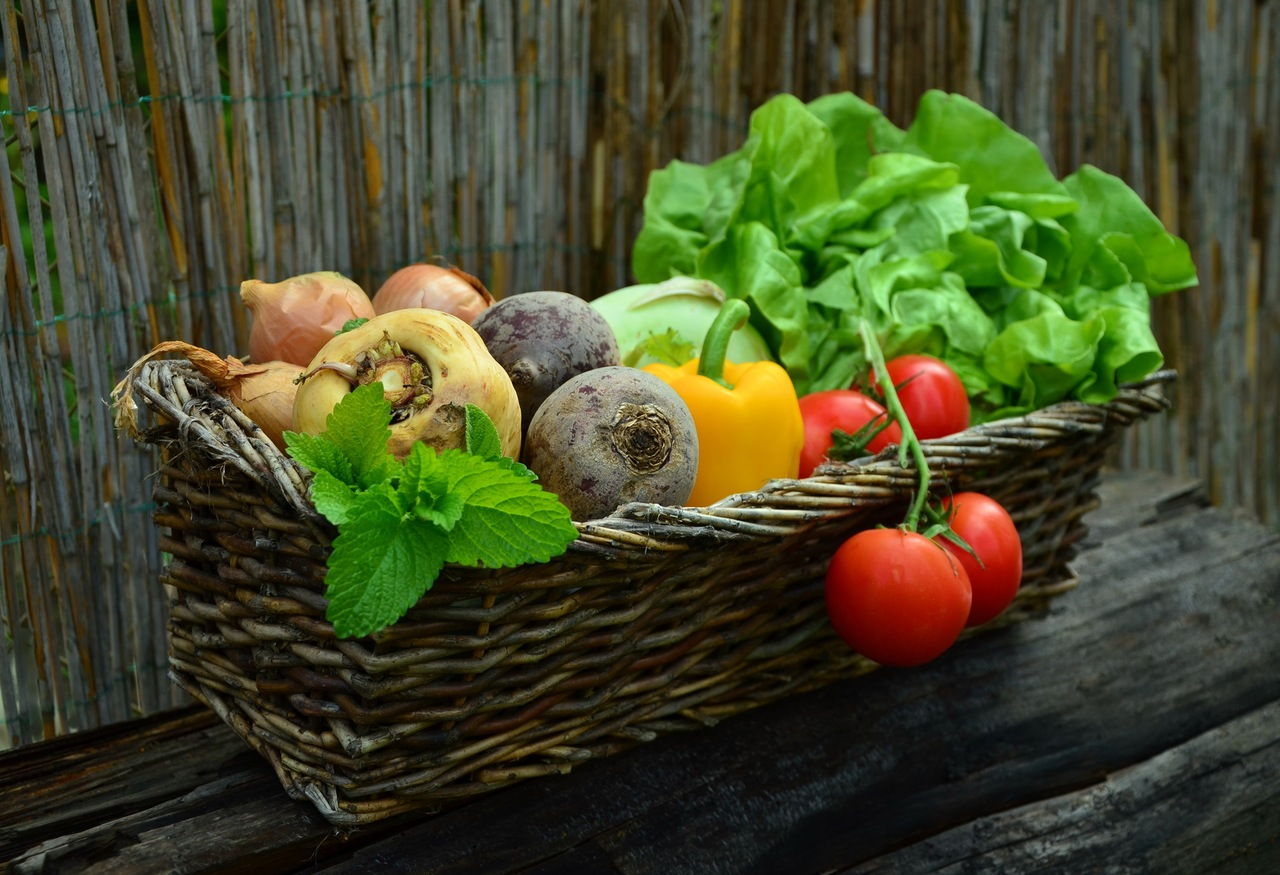
\includegraphics[width=\textwidth]{images/opening}\par
\sffamily\bfseries\Large\@author\par
\bigskip\medskip
{\color{color2}\normalfont\normalsize\textbf{Summary:}\\
\getsummary}
\end{center}
\clearpage
}
\makeatother
%%%

%%% fancy boxes
\usepackage{tcolorbox}
\usepackage{wrapfig}
\def\fullboxbegin{
\bigskip
\begin{tcolorbox}[colback=color1,colframe=color1,coltext=white,arc=0mm,boxrule=0pt]
}
\def\fullboxend{\end{tcolorbox}\medskip}
%
\def\leftboxbegin{
\begin{wrapfigure}{l}{0.5\textwidth}
\begin{tcolorbox}[colback=color1,colframe=color1,coltext=white,arc=0mm,boxrule=0pt]
}
\def\leftboxend{
\end{tcolorbox}
\end{wrapfigure}
}
%
\def\rightboxbegin{
\begin{wrapfigure}{r}{0.5\textwidth}
\begin{tcolorbox}[colback=color1,colframe=color1,coltext=white,arc=0mm,boxrule=0pt]
}
\def\rightboxend{
\end{tcolorbox}
\end{wrapfigure}
}
%
\newcounter{frames}
\def\frameboxbegin#1{
\bigskip
\refstepcounter{frames}
\begin{tcolorbox}[colback=white,colframe=color1,arc=0mm,title={\MakeUppercase{\textbf{Frame \arabic{frames}}: #1}}]
}
\def\frameboxend{
\end{tcolorbox}
}
%%%

%custom Requirements titles
\usepackage{titlesec}
%\usepackage{hyperref}
%Funtional
\titleclass{\requirement}{straight}[\subsubsection]
\newcounter{requirement}
\titleformat{\requirement}
  {\color{color1}\sffamily\bfseries}{}{0em}
  {\refstepcounter{requirement}FR \therequirement:~}
\titlespacing*{\requirement}{0pt}{3.25ex plus 1ex minus .2ex}{1.5ex plus .2ex}

\setcounter{tocdepth}{4}
\makeatletter
  \def\toclevel@requirement{5}
  \def\l@requirement{\@dottedtocline{5}{3.8em}{3.2em}}
\makeatother
%%%


%requirements table enviromnent
\newenvironment{reqtable}
{
    \medskip
    \begin{tabular}{|p{3.5cm}|p{11cm}|}
    \hline
}
{\end{tabular}}


\usepackage{lipsum}

%%%%%%%%%%%%%%%
% Title Page
\title{Cupboard:\\Requirements Specfication}
\author{Team 8:\\Clare Doran, Abdul Ghani, Ucizi Mafeni, Luke Needham, Soumya Singh}
\date{\today}
\summary{
A web app built with the intention of helping reduce food waste
}
%%%%%%%%%%%%%%%

\begin{document}
\maketitle

\tableofcontents
\clearpage
%glossary
%define "active" listing
%define listing
%define immutable
%define trade
\section{Introduction}
7 million tonnes of food goes to waste in the UK, more than half of which is 
edible (https://www.lovefoodhatewaste.com/node/2472).
Meanwhile,  many people throughout the country struggle to put together enough 
money for food, with food banks becoming busier every year
(https://www.trusselltrust.org/2015/11/18/uk-foodbank-use-still-at-record-levels-as-hunger-remains-major-concern-for-low-income-families/)

Cupboard aims to be a system that allows users to painlessly find and share food
that would otherwise go to waste. It should be quick and easy to use as it is
too easy to just throw away food. 
It will also allow users to arrange collection in a manner that does not force
them to disclose their house address or any other details they wish to keep
private.


\section{Project Scope}
Cupboard will facilitate the sharing of food between users. It will do so in a
manner that is as simple as possible, as we want to discourage people from
taking the easy route of simply binning food they wont eat.
There will be a simple points-based system and a ranking system in order to
encourage sharing of food and reassure other users that the quality of food is
likely to be good. When some food has been ‘successfully exchanged’ both
parties will get points and will be able to rate each other. If users wish to
participate, there will be a simple public leaderboard.
Users can set their dietary requirements (allergies, religious etc.) and have
results automatically filtered. 
There will be a messaging system (in order to arrange collection) and a comments
system (in order to view interest in the item and ask questions).


\section{Domain Analysis}
There are a couple of examples of food sharing sites/apps such as:
\begin{itemize}
    \item foodsharing.de(https://foodsharing.de/): A German food sharing site
        that allows users (just like our site) to trade food that is going out
        of date with other users to reduce food waste.
        However it is only available in Germany.
    \item Olio (https://olioex.com/): Mobile app with strong UK presence.
        A key distinguishing feature is "Drop Boxes".
        These are local stores/cafes where users can drop off food they'd like
        to be shared.
    \item SharingFood
        (https://itunes.apple.com/us/app/sharing-food/id992111062?mt=8):
        Mobile app based in Italy.
        Seems to be fairly new and so has a very small user base.
\end{itemize}


\section{Proposed Deliverables}
(Gantt Chart Goes here)

\section{Identified, Risks, Assumptions, Dependencies and Constraints}
\begin{itemize}
    \item User Location: How much information about the user's location can we
        make publicly available without putting their security ar risk?
    \item Assuming google maps should be able to find the addresses entered by
        the user.The location functionality is completely dependent on the
        Google Maps API.
\end{itemize}

\section{Solution Requirements}
\subsection{Functional Requirements}
%move section of speech to development approach
N.B. Due to the highly time-sensitive nature of the project, any low priority
requirements (and thier linked dependencies) may not be implemented.
As such, all low priority requirements are inherently unessential to the
system, and it will remain fully operational with or without them.

\requirement{Error-Reporting System}
\label{fr:error-reporting}

\requirement{User Feedback System}
\label{fr:error-reporting}

\requirement{User sign up}
\label{fr:user-sign-up}

\begin{reqtable}
    Description        & The User should be able to create an account by 
                        following the registration process.\\
    \hline
    Priority           & High\\
    \hline
    Dependencies       &  Get User Registration Details\\
    \hline
    Expected results   & Following account creation, the user will be able to 
                        login using their provided username and password\\
    \hline
    Exception Handling & \\
    \hline
\end{reqtable}

\requirement{Get User Registration Details}
\label{fr:registration-details}

\begin{reqtable}
    Description        & During sign-up, the user should provide the following
                        details in order to successfully complete the sign-up
                        process:

                        \begin{itemize}
                            \itemsep-1em
                            \item username (must be unique)
                            \item email address
                            \item password
                            \item physical address
                            \item post code (must be valid)
                        \end{itemize}
                        
                        In addition, the user should also be given the option
                        to fill in their Dietary Requirements and Allergy 
                        Information. However, it is not mandatory to fill in 
                        these details in order to complete registration.

                        \\
    \hline
    Priority           & High\\
    \hline
    Dependencies       & Validate User Details, Dietary Requirements, 
                        Allergy Information\\
    \hline
    Expected results   & User inputs all valid fields and proceeds to complete
                        registration\\
    \hline
    Exception Handling & Refer to val\\
    \hline
\end{reqtable}

\requirement{Validate Registration Details}
\label{fr:validation}

\begin{reqtable}
    Description        & Information in the registration form should be
                        validated as follows:
                        
                        username: checked against database to see if its unique

                        email-address: adheres to general email structure 
                        (<someuser>@<somehost>.<com/net\ldots>)

                        password: minimum length of 7 characters, alphanumeric,
                        contains one symbol from valid symbol list
                        (refer to glossary)

                        postcode: is actual valid postcode 
                        (check in UK postcode directory)

                        If there exists an invalid input on submission,
                        the form must be rejected and the user must be
                        notified of their error
                        (i.e highlight incorrect field and place error message
                        next to it)
                        \\
    \hline
    Priority           & High\\
    \hline
    Dependencies       & User Reg\\
    \hline
    Expected results   & Validation system correctly highlights any invalid
                        fields\\
    \hline
    Exception Handling & N.A.\\
    \hline
\end{reqtable}

\requirement{Account Activation}
\label{fr:activation}

\begin{reqtable}
    Description        & 
                        Once the user has provided the registration details,
                        an email with an account activation link
                        will be sent to the provided email address. The user
                        should then be able to follow the activation link in
                        order to activate their account.\\
    \hline
    Priority           & Low \\
    \hline
    Dependencies       & User Reg\\
    \hline
    Expected results   & After the user follows the activation link,
                        they should be able to login to their account using
                        the login details they provided during registration\\
    \hline
    Exception Handling & Activation link doesn't work: the user should have the
                        option to request another activation link.

                        Incorrect email address provided: the user will have the
                        option to correct the provided email address.\\
    \hline
\end{reqtable}

\requirement{User Dashboard}
\label{fr:user-dashboard}

\begin{reqtable}
    Description        & Following login, all registered users should have
                        access to a personal
                        dashboard where they can do the following:
                        
                        \begin{itemize}
                            \itemsep-1em
                            \item edit their personal details
                            \item edit their current dietary requirements
                        \end{itemize}

                        \\
    \hline
    Priority           & High\\
    \hline
    Dependencies       & Edit Profile, Privacy Settings,
                        Edit Dietary Requirements\\
    \hline
    Expected results   & User is able to access and edit all personal
                        information from the dashboard\\
    \hline
    Exception Handling & Registered and logged-in user can't access dashboard:
                        notify webmaster of error
                        \\
    \hline
\end{reqtable}


\requirement{Edit Profile}
\label{fr:edit-profile}

\begin{reqtable}
    Description        & A user should be able to change their personal details
                        this includes:

                        \begin{itemize}
                            \itemsep-1em
                            \item their username
                            \item their email address
                            \item their password
                            \item their dietary requirements
                            \item their allergy information
                        \end{itemize}

                        All changes to personal details will be validated under
                        the standards mentioned in
                        (Validate Registration Details).

                        With regards to dietary requirements and allergy
                        information, users will be able to select whichever
                        categories listed in (Dietary Requirements) and
                        (Allergy Information) that personally apply to them.
                        \\
    \hline
    Priority           & High\\
    \hline
    Dependencies       & Validate Registration Details, Dietary Requirements,
                        Allergy Information\\
    \hline
    Expected results   & User able to successfully change personal details.\\
    \hline
    Exception Handling & New details don't satisfy validation standards:
                        Invalid fields must be highlighted with hint
                        (as to why field is Invalid) shown
                        
                        User unable to save changes: Report error to webmaster\\
    \hline
\end{reqtable}


\requirement{Dietary Requirements}
\label{fr:dietary-requirements}

\begin{reqtable}
    Description        & By default, dietary requirements will be split into
                        the following categories:

                        \begin{itemize}
                            \itemsep-1em
                            \item Halal
                            \item Kosher
                            \item Vegan
                            \item Vegetarian
                        \end{itemize}

                        There will be an additional category group called 
                        "other" where users can specify a dietary requirement
                        not listed in the default categories.
                        \\
    \hline
    Priority           & High\\
    \hline
    Dependencies       & \\
    \hline
    Expected results   & \\
    \hline
    Exception Handling & \\
    \hline
\end{reqtable}


\requirement{Allergy Information}
\label{fr:allergy-information}

\begin{reqtable}
    Description        & By default, allergies will be split into
                        the following categories:

                        \begin{itemize}
                            \itemsep-1em
                            \item Peanuts
                            \item Gluten
                            \item Lactose
                            \item Soy
                        \end{itemize}

                        There will be an additional category group called 
                        "other" where users can specify any allergies not listed
                        in the default categories.\\
    \hline
    Priority           & High\\
    \hline
    Dependencies       & \\
    \hline
    Expected results   & \\
    \hline
    Exception Handling & \\
    \hline
\end{reqtable}

\requirement{Listing}
\label{fr:listing}

\requirement{Listing Status}
\label{fr:listing-status}

\requirement{Active Listing}
\label{fr:active-listing}

\requirement{Inactive Listing}
\label{fr:inactive-listing}


\requirement{Listings Page}
\label{fr:listings-page}

\begin{reqtable}
    Description        & Any Logged-in user should have access to a personal 
                        listings page, from where they can do the following:
                        
                        \begin{itemize}
                            \itemsep-1em
                            \item view thei1
                            \item 
                            \item 
                        \end{itemize}
                        \\
    \hline
    Priority           & \\
    \hline
    Dependencies       & \\
    \hline
    Expected results   & \\
    \hline
    Exception Handling & \\
    \hline
\end{reqtable}

\requirement{Comments Board}
\label{fr:comments}
\requirement{Item Catalogue}
\label{fr:item-catalogue}

\requirement{Search}
\label{fr:search}

\requirement{Sorting Search Results}
\label{fr:sorting}

\requirement{Search Filters}
\label{fr:filters}

\requirement{User’s Past \& Current Listings Page}
\label{fr:user-listing-page}

\requirement{Add Listing}
\label{fr:add-listing}

\requirement{Edit Listing}
\label{fr:edit-listing}

\requirement{Commit to collect}
\label{fr:commit}

\requirement{Messaging}
\label{fr:messaging}

\requirement{Orders Page}
\label{fr:orders}

\requirement{Watch-list}
\label{fr:watchlist}

\requirement{User Score}
\label{fr:user-score}

\requirement{User Ratings}
\label{fr:user-ratings}


\subsection{Non-Functional Requirements}
\begin{itemize}
    \item Items will be stored in only one location and so will be consistent.
    \item Animations and transitions will be simple and fluent in order to keep
        the interface responsive.
    \item All functionalities will be supported on all devices, apart from
        wearables.
\end{itemize}


\section{Development Approach}

\subsection{Key Summary}
We've decided to use PHPStorm as the main IDE. Ultimately we hope to host the
Database (and possibly website) on AWS. We will mainly collaborate using
Github and Slack (and occasionally email).

Though we'll all inevitably contribute to both sides of the site, we've
decided to split the work as follows:
\begin{itemize}
    \item \textbf{Design and Frontend:} Clare, Ucizi and Luke
    \item \textbf{Database and Backend:} Soumya and Abdul
\end{itemize}

\subsection{Development Stack}
\begin{itemize}
    \item PHP (Database and other backend features)
    \item HTML/CSS
    \item SQL
    \item Javascript (Client-side features)
    \item Bootstrap (Simplifies mobile compatibility)
    \item Git
\end{itemize}


\section{References}
\end{document}
